\documentclass[12pt, a4paper]{article}   % font size, paper size

% Encoding & language
\usepackage[utf8]{inputenc}
\usepackage[T1]{fontenc}
\usepackage[english]{babel}
% LTeX: language=en-GB

% Page layout
\usepackage[margin=2.5cm]{geometry}

% Math
\usepackage{amsmath}    % extended math environments
\usepackage{amssymb}    % extra symbols (ℝ, ∞, etc.)
\usepackage{amsthm}
\newtheorem{theorem}{Theorem}

% Graphics & figures
\usepackage{graphicx}   % \includegraphics
\usepackage{float}      % [H] placement option
\usepackage{subcaption}

% Tables
\usepackage{booktabs}   % \toprule, \midrule, \bottomrule
\usepackage{siunitx}

% Hyperlinks (load last)
\usepackage[hidelinks]{hyperref}

\usepackage[backend=biber, style=mla]{biblatex}
\addbibresource{MathematicsExtendedEssay.bib}

\usepackage{csquotes}

\usepackage{verbatim}

\usepackage{tikz}
\usetikzlibrary{graphs, positioning, calc}

%TC:macro \section [ignore]
%TC:macro \subsection [ignore]
%TC:macro \subsubsection [ignore]

% ---- Document metadata ----
\title{Mathematics Extended Essay on the Topic of Clique Sizes in Scale Free Networks}
\author{Personal Code: mmv147}
\date{\today}  
\graphicspath{ {./images/} }
\begin{document}

\maketitle
\begin{center}
    \textbf{Word count:} 2780
    \par
    \bigskip
    \bigskip
    \textbf{Research Question}: How does the power coefficient \( \gamma \) affect \par maximum clique sizes in scale free networks at the edge of admissibility?
\end{center}

\newpage
%TC:ignore
\tableofcontents
%TC:endignore
\newpage

\section{Introduction}
% -	A brief introduction
% -	My motivation to explore this topic

My AI HL maths course focuses little on a mathematical branch called discrete mathematics. Never having understood the underlying field of study, and knowing that we would cover very little of it in the AI HL syllabus, I was interested in exploring it further. I looked into randomization, graph theory, probabilities, algorithm design and finally landed on Erdős’ Probabilistic Method. Fascinated by the concept of non-constructive proofs, my understanding followed closely by my curiosity increased rapidly which led me to what I quickly realised was the frontier of mathematics. Only understanding very little but eager to learn I continued researching. 

This extended essay is a summary of these findings and an attempt at combining two inherently close concepts that I could find little definitive information on in my research: how clique sizes relate to the power-law distribution of scale free networks. In other words, I will answer the question: How does the power coefficient \( \gamma \) affect maximum clique sizes in scale free networks at the edge of admissibility?

Clique sizes are parts of graphs (from graph theory, not Cartesian planes) where all nodes are interconnected with one another. Scale free networks are graphs where the number of connections all nodes have follows the shape of a power function: \(f(x)=x^{-\gamma}\). In other words, there are many nodes with few connections and a few with many. The shape of the function means a scale free network has few \textit{hubs} which are much more connected than the majority of other nodes, such as the one below with the two dark blue nodes:

\begin{figure}[H]
\centering
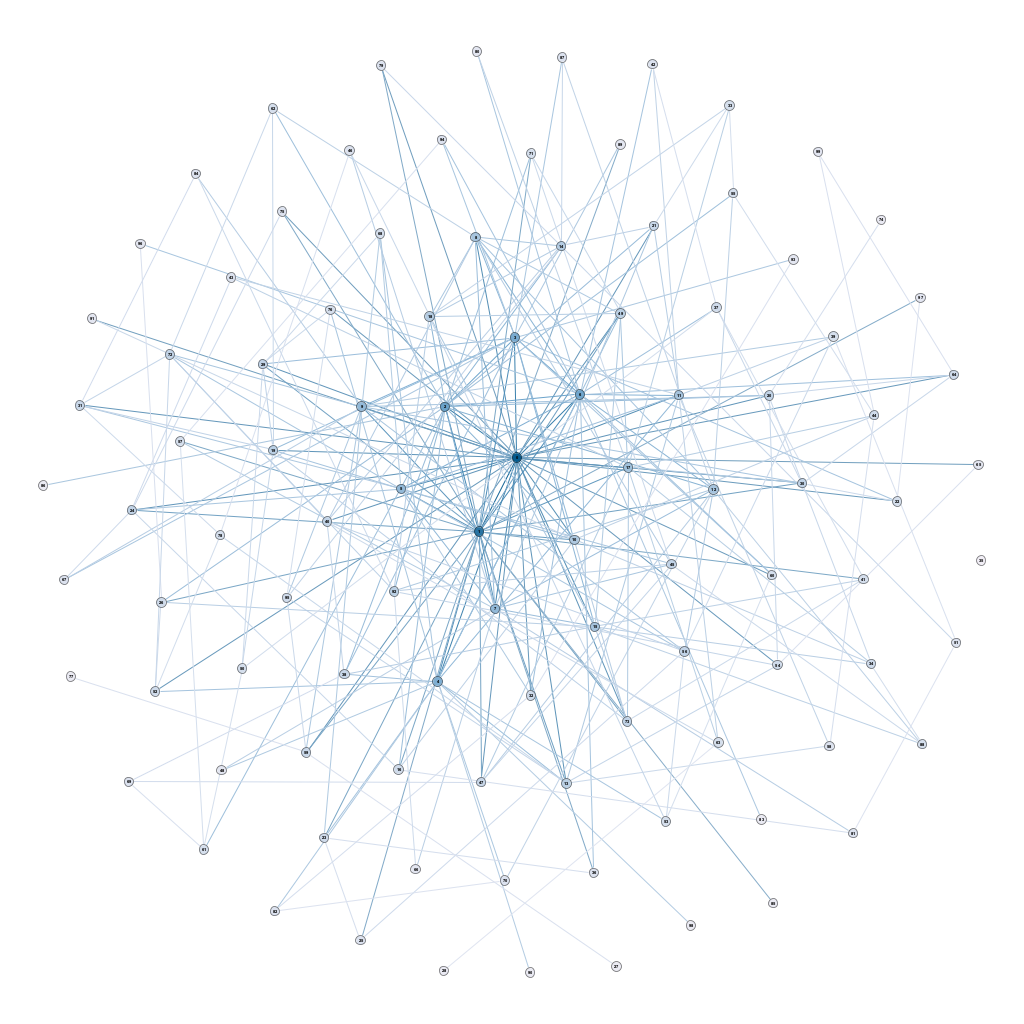
\includegraphics[width=0.48\textwidth]{exampleScaleFree.png}
\caption{Caption text here}
\label{fig:my-image}
\end{figure}

Scale free networks are remarkable graphs because they can be found and are made use of in every corner of our lives. They are defined by their nodes' degree, which I will define later, but even without the mathematical knowledge they are conceptually interesting. The internet and Instagram are scale free networks. Telecommunications networks are scale free. Most modern financial networks have hubs. Any network which makes use of a few hubs that have many more connections than the rest is likely a scale free network. The simple fact that there are many tangible examples to understand the concept make this topic fascinating to explore. \autocite{ScalefreeNetwork2026}

This essay will be structured into three main parts. First, I will explain the knowledge I acquired through my research to a level a Maths AI HL student can understand. I will look at the concept of binomial coefficients, the generation of random graphs and specifically scale free networks, and present the basics of the probabilistic method. Second, using these tools, I will present a derivation of the relationship between the exponent \( \gamma \) in distribution of node degrees and the clique sizes found in a predefined graph. Finally, I will investigate patterns formed through the empirical generation of scale free networks.

%To briefly help the reader to understand this essay better, below are a few definitions and pointers on notation which might be useful throughout the next few pages:
% \begin{description}
%     \item[Object] The concept of an object is a highly philosophical matter, yet for the purpose of this essay, the reader can assume that it is simply an abstract \textit{thing}. It can be anything from a number, a node of a graph or a name on a list. \autocite{MathematicalObject2026}
%     \item[Set] A set is a collection of such \textit{things}, i.e. objects.
%     \item[Element] An element is a distinct object in a set.
%     \item[ s \( \in \) S ] This notation (\( \in \)) will come up frequently and means "s is an element of S".
%     \item[Binomial Coefficient] The notation of a binomial coefficients will be discussed in the next section.
% \end{description}


\section{Scale Free Networks and Graph Theory}
% -	Describing the concept of graphs
% -	Defining terms
% -	Applying the idea to scale free networks

One predominant branch of Mathematics which is often ignored is called discrete mathematics. It focuses on the study of countable objects. Part of discrete mathematics is the study of graphs which is known as graph theory. These should not be confused with a graph on a Cartesian plane. These graphs allow the mathematical analysis of networks and connections, like streets, mobile networks, or social media networks. From now on the use of the word graph will refer to the mathematical graph which makes part of discrete mathematics, i.e. a network of nodes connected by edges.

\subsection{Definitions}

For clarity, I will define the following terms, as they are different around the mathematical world:
\begin{description}
    \item[Node:] A node is the same as a vertex and is the indivisible point at which one or more edges meet. \autocite{VertexGraphTheory2026}
    \item[Edge:] An edge is the connection between nodes. \autocite{GlossaryGraphTheory2026}
    \item[Degree:] The degree of a node is the number of connections, i.e. edges, it has to another node. In general, this essay will denote it as \( k \) to simplify understanding. \autocite{GlossaryGraphTheory2026}
    \item[Complete Graph]  A graph in which every pair of distinct nodes is connected by an edge. It will be denoted as \( K_n \) where n is the number of nodes in the graph. \autocite{DegreeGraphTheory2026}
    \item[Subgraph] A subgraph is a subset of nodes of a graph and all the edges connecting pairs of the subset. This creates a new graph "inside" another graph.\autocite{GlossaryGraphTheory2026}
    \item[Clique] A clique is a tighter definition of a subgraph as it requires the subgraph to be complete. \autocite{CliqueGraphTheory2025}
\end{description}


I am only making use of simple undirected graphs, meaning that there can only be a single edge between every node and that the edges do not represent a direction in the connection between nodes (as would be required when representing one-way streets for example) \autocite{GraphDiscreteMathematics2026}.
\subsection{Scale Free Networks} \label{sec:scale-free-networks}

This extended essay will investigate scale free networks which are representative of many real-world networks because of their "Hubs". A scale free network gives a power a relation between the degree of a node and the probability of its occurrence. In other words, 
\begin{equation} \label{eq:proportional-scale-free}
    P(k) \propto k^{-\gamma}
\end{equation}
where \( \gamma \) is some exponent and \( P(k) \) the probability that a node has degree \( k \) \autocite{ScalefreeNetwork2026}.

To generate scale free networks, different methods exist. The most commonly used model is called \textit{configuration model} because it allows the degree of every node to be pre-defined \autocite{ConfigurationModel2025}. Since scale free networks are defined by the distribution of a graph's nodes' degree, that is a requirement. When it is of interest to fix the degree sequence exactly it is possible to make use of a microcanonical model which defines the exact degree of every node in the graph and randomly draws edges according to these requirements \autocite{ConfigurationModel2025}. The diagram below shows how every node has a predefined degree and only the exact connections are generated randomly.
\begin{figure}[H]
\centering
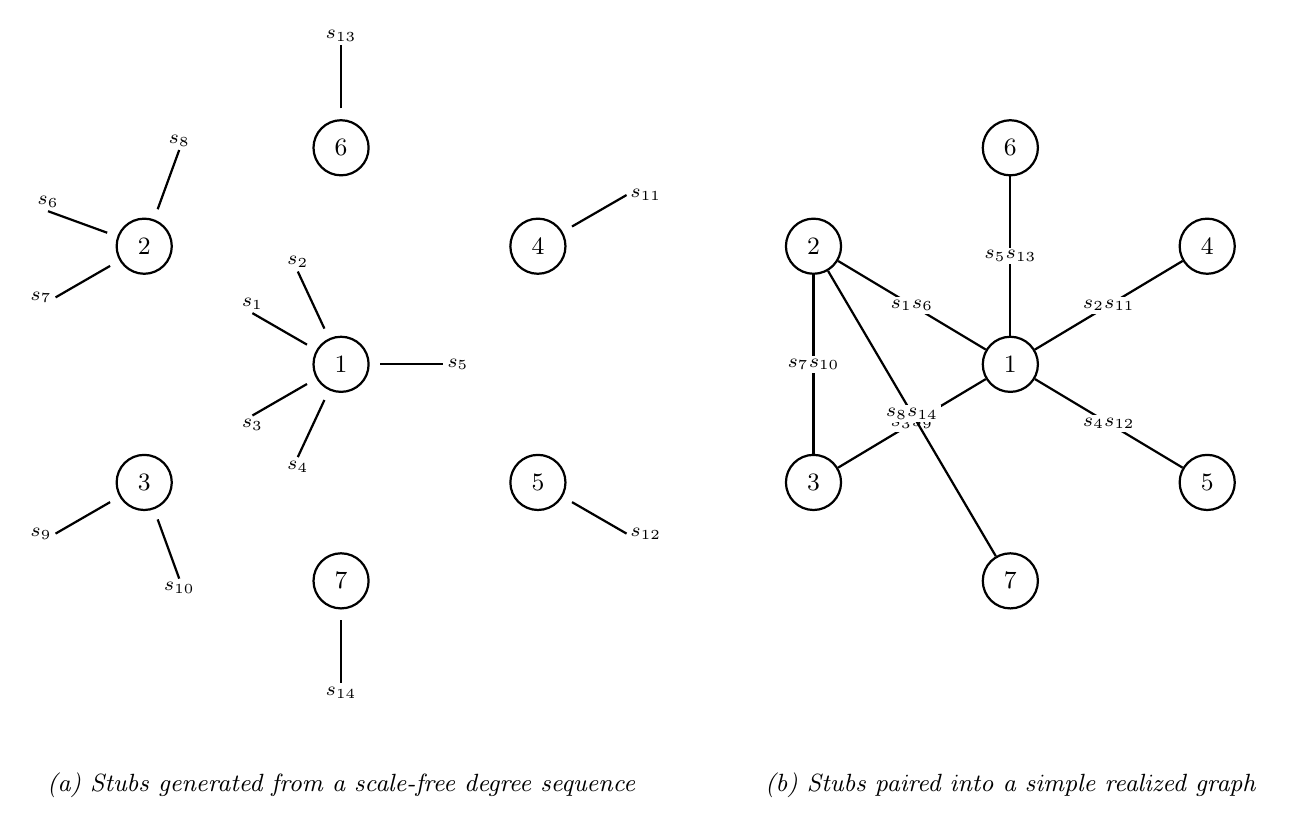
\begin{tikzpicture}[
    vertex/.style={circle, draw=black, fill=white, thick, minimum size=7mm, font=\small},
    stub/.style={thick},
    stublabel/.style={font=\scriptsize, inner sep=1pt},
    edgeline/.style={thick, -},
    edgelabel/.style={font=\scriptsize, fill=white, inner sep=1pt}
]

%=== PANEL 1: Vertices with unmatched stubs ===
\begin{scope}
    \node[vertex] (A) at (2.5,0)    {1}; % hub, degree 5
    \node[vertex] (B) at (0,1.5)    {2}; % degree 3
    \node[vertex] (C) at (0,-1.5)   {3}; % degree 2
    \node[vertex] (D) at (5,1.5)    {4}; % degree 1
    \node[vertex] (E) at (5,-1.5)   {5}; % degree 1
    \node[vertex] (F) at (2.5,2.75) {6}; % degree 1
    \node[vertex] (G) at (2.5,-2.75){7}; % degree 1

    % Stubs for hub 1 (5), labelled s1-s5
    \draw[stub] (A) ++(150:5mm) -- ++(150:8mm) node[stublabel, above]{\(s_1\)};
    \draw[stub] (A) ++(115:5mm) -- ++(115:8mm) node[stublabel, above]{\(s_2\)};
    \draw[stub] (A) ++(-150:5mm)-- ++(-150:8mm) node[stublabel, below]{\(s_3\)};
    \draw[stub] (A) ++(-115:5mm)-- ++(-115:8mm) node[stublabel, below]{\(s_4\)};
    \draw[stub] (A) ++(0:5mm)   -- ++(0:8mm)   node[stublabel, right]{\(s_5\)};

    % Stubs for 2 (3), labelled s6-s8
    \draw[stub] (B) ++(160:5mm) -- ++(160:8mm) node[stublabel, above]{\(s_6\)};
    \draw[stub] (B) ++(210:5mm) -- ++(210:8mm) node[stublabel, left]{\(s_7\)};
    \draw[stub] (B) ++(70:5mm)  -- ++(70:8mm)  node[stublabel, above]{\(s_8\)};

    % Stubs for 3 (2), labelled s9-s10
    \draw[stub] (C) ++(210:5mm) -- ++(210:8mm) node[stublabel, left]{\(s_9\)};
    \draw[stub] (C) ++(-70:5mm) -- ++(-70:8mm) node[stublabel, below]{\(s_{10}\)};

    % Stub for 4 (1), labelled s11
    \draw[stub] (D) ++(30:5mm)  -- ++(30:8mm)  node[stublabel, right]{\(s_{11}\)};

    % Stub for 5 (1), labelled s12
    \draw[stub] (E) ++(-30:5mm) -- ++(-30:8mm) node[stublabel, right]{\(s_{12}\)};

    % Stub for 6 (1), labelled s13
    \draw[stub] (F) ++(90:5mm)  -- ++(90:8mm)  node[stublabel, above]{\(s_{13}\)};

    % Stub for 7 (1), labelled s14
    \draw[stub] (G) ++(-90:5mm) -- ++(-90:8mm) node[stublabel, below]{\(s_{14}\)};

    \node[below=32mm of C, xshift=25mm, font=\small\itshape]
        {(a) Stubs generated from a scale-free degree sequence};
\end{scope}

%=== PANEL 2: Same vertices, stubs paired into a simple realized graph ===
\begin{scope}[xshift=8.5cm]
    \node[vertex] (A2) at (2.5,0)    {1};
    \node[vertex] (B2) at (0,1.5)    {2};
    \node[vertex] (C2) at (0,-1.5)   {3};
    \node[vertex] (D2) at (5,1.5)    {4};
    \node[vertex] (E2) at (5,-1.5)   {5};
    \node[vertex] (F2) at (2.5,2.75) {6};
    \node[vertex] (G2) at (2.5,-2.75){7};

    % Matching: 1-2, 1-3, 1-4, 1-5, 1-6, 2-3, 2-7
    \draw[edgeline] (A2) -- (B2);
    \node[edgelabel] at ($(A2)!0.5!(B2)$) {\(s_1s_6\)};
    \draw[edgeline] (A2) -- (C2);
    \node[edgelabel] at ($(A2)!0.5!(C2)$) {\(s_3s_9\)};
    \draw[edgeline] (A2) -- (D2);
    \node[edgelabel] at ($(A2)!0.5!(D2)$) {\(s_2s_{11}\)};
    \draw[edgeline] (A2) -- (E2);
    \node[edgelabel] at ($(A2)!0.5!(E2)$) {\(s_4s_{12}\)};
    \draw[edgeline] (A2) -- (F2);
    \node[edgelabel] at ($(A2)!0.5!(F2)$) {\(s_5s_{13}\)};
    \draw[edgeline] (B2) -- (C2);
    \node[edgelabel] at ($(B2)!0.5!(C2)$) {\(s_7s_{10}\)};
    \draw[edgeline] (B2) -- (G2);
    \node[edgelabel] at ($(B2)!0.5!(G2)$) {\(s_8s_{14}\)};

    \node[below=32mm of C2, xshift=25mm, font=\small\itshape]
        {(b) Stubs paired into a simple realized graph};
\end{scope}

\end{tikzpicture}
\label{fig:configuration-model-stubs}
\end{figure}


On the other hand, a canonical model works with the probability distributions of the edges in a network. The one this extended essay focuses on is the Chung-Lu (canonical) Configuration Model because the probabilistic generation is also easier to analyse using the probabilistic method which we will get into below. \autocite{ScalefreeNetwork2026}

In short, the model defines the probability of an edge between two nodes \( v_h \) and \( v_j \) to be:

\begin{equation} \label{eq:chung-lu-conf-model}
    p_{hj} = \frac{w_h w_j}{\sum_{i}{w_i}}
\end{equation}
where \( p_{hj} \) is the probability, \( w_h \) and \( w_j\) are weights associated with every node, and \(\sum_{i}{w_i}\) is the sum of all weights \autocite{chungAverageDistancesRandom2002}. These \textit{weights} are generated beforehand and assigned to every node. They are also called a node's expected degree, since the larger the weight the greater the degree and the two are directly proportional. If we hypothetically double \( w_h \) in equation \ref{eq:chung-lu-conf-model} then the probability of a degree getting generated doubles, since:

\[
 \frac{(2 \times w_h) w_j}{\sum_{i}{w_i}} = 2 \times p_{hj}
\]

We therefore expect the node to have double the degree.

We divide by the sum of all weights because we are working with probabilities and as such, require our values to be normalised. This step is also required when calculating the probability of rolling a 5 when throwing a fair 6-sided dice for example. There is 1 side with 5 eyes, and 6 sides in total, therefore the probability of rolling a 5 is \( \frac{1}{6} \). 

\textcite{chungAverageDistancesRandom2002} explicitly define their graph as G(\textbf{w}) where \textbf{w} is the expected degree sequence. This is standard notation in the field of graph theory and should only serve a reader with a basic understanding as a reference point. It is important to note that the expected degree sequence are the weights from before.

To generate a graph with the \textcite{chungAverageDistancesRandom2002} model, we therefore need to generate the weight sequence first. In the case of scale free networks, these weights need to follow the proportionality from equation \ref{eq:proportional-scale-free} above. To make the model work, however, it is further stated that all probabilities are independent and that for the greatest i, \( w_i^2 < \sum_{i}{w_i}\) \autocite{chungAverageDistancesRandom2002}. In other words, if we take two nodes with the greatest weight, their product cannot be greater than the sum of all weights. After all, the probability of an edge generating cannot be greater than 1, which would be the case if \( w_h w_j > \sum_{i}{w_i}\) in the equation \( \frac{w_h w_j}{\sum_{i}{w_i}} \).

Bringing the power law distribution and the weight requirements together, we come to this equation, originally published by Chung and Lu and adapted to the notation consistent in this essay. 

\begin{equation} \label{eq:weight-generation-equation}
    w_i = w_{\text{max}} \times i^{ -\frac{1}{\gamma-1}}
\end{equation}

Where \( w_{\text{max}} \) is the maximum weight, \( i \) is the rank, and \( \gamma \) the power law exponent \autocite{chungAverageDistancesRandom2002}. The rank defines the position in the degree sequence. An attentive reader might notice how the power coefficient is not exactly \(-\gamma\) but instead \(-\frac{1}{\gamma-1}\). The reason why is beyond the scope of this essay, but in short, it has to do with the fact that one is a function of the degree (\(P(k) \propto k^{-\gamma}\)) and the other a function of the rank (\( w_i = w_{\text{max}} \times i^{ -\frac{1}{\gamma-1}}\)).

Choosing the maximum weight is best done by calculating the maximum value permitted by the equality \( w_i^2 \leq \sum_{i}{w_i}\), after all, a normalised weight should not exceed a probability of \( 1 \). To find \( w_{\text{max}} \) we need to take apart the equation summing all weights:

\begin{equation} \label{eq:S-and-T-definition}
\begin{aligned}
S &= \sum_{i}{w_i} \\
  &= \sum_{i}{w_{\text{max}} \times i^{ -\frac{1}{\gamma-1}}} \\
  &= w_{\text{max}} \times \sum_{i}{i^{ -\frac{1}{\gamma-1}}} \\
  &= w_{\text{max}}T
\end{aligned}
\end{equation}

where \( S \) and \( T \) are chosen to keep the notation clean below. With this information, we can now apply the inequality:

\[
w_i^2 \leq \sum_{i}{w_i} = w_{\text{max}}^2 \leq\sum_{i}{w_i}  = w_{\text{max}}^2 < S
\]   

In turn simplifying to:
\[
w_{\text{max}}^2 \leq S = w_{\text{max}}T
\] 

If we divide by \(w_{\text{max}}\), since \(w_{\text{max}} > 0\):
\[ 
w_{\text{max}} \leq T
\]   

And, as a reminder:
\[
T = \sum_{i}{i^{ -\frac{1}{\gamma-1}}}
\]   

Therefore:
\begin{equation} \label{eq:wmax-leq-T}
w_{\text{max}} \leq \sum_{i}{i^{ -\frac{1}{\gamma-1}}}
\end{equation}


In other words, with \(n\) and \(\gamma\) we can compute the probabilistic limit to the weights of the sequence which we can use to generate random scale free networks.




\section{Combinations and Permutations} \label{sec:combinations-permutations}

This essay will touch into the probabilistic method. To do so, it is important to clarify the concept of what are colloquially known as \textit{combinations}. Imagine a simple cake in which all ingredients are mixed independent of the order. In mathematical language, that is called a combination of objects. If, on the other hand, the order matters, like for a phone password, that is called a permutation. There is a further distinction between a combination and permutation where repeats are allowed or not. A phone password, for example, can have repeating digits, arranging the winners of a race, on the other hand, cannot. 
\autocite{CombinationsPermutations}

\subsection{Permutations with Repetitions}

Calculating possible arrangements of objects depends on the requirements. It is simplest to calculate all possible permutations when repetitions are allowed. If we have a 4-digit phone password where every digit can be a digit from 0-9 with repetitions there are: \[ 10 \times 10 \times 10 \times 10 = 10^{4} = 10000 \] possible permutations since every new digit we can choose from another set of 10 numbers. 

Generalising, if we have \(n\) different types in a specific order of \(r\) items with repetitions allowed, we can assume there are: 
\begin{equation} \label{eq:permutations-with-repetition}
n^{r}
\end{equation}
permutations.

\subsection{Permutations without Repetitions}

If, however, we cannot have repeating values, because we are working with all the possible results of a race, we have to decrease the pool of objects to pick from with every step. When repetitions were allowed, we could multiply the same number over and over. This time, however, we need to calculate the possibilities from a decreasing number of choices. Taking 7 runners in a race, there are 7 options to be first, but then only 6 to come second, then 5 and so on. There are therefore \[7 \times 6 \times 5 \times 4 \times 3 \times 2 \times 1 = \] possibilities. Mathematically, this can be denoted as \(7!\). If want to choose the first three winners only we would multiply \(7 \times 6 \times 5\). Since our notation goes until 1 however, we can cancel out the latter part: 

\[ \frac{7 \times 6 \times 5 \times 4 \times 3 \times 2 \times 1}{4 \times 3 \times 2 \times 1} = \frac{7!}{4!}\]

Generalising, if we chose \(r\) items from \(n\) different types where repetitions are not allowed we get:
\begin{equation} \label{eq:permutations-without-repetition}
\frac{n!}{(n-r)!}
\end{equation} 

\subsection{Combinations without Repetitions}

If we apply this idea to combinations where there are no repetition, in other words we do not care about the order but cannot have duplicates, we need to remove all duplicates. Taking our race example, if we only care about the all the possible ways we can list 3 different athletes outwe can generate, independent of their order, we have to remove all the ways in which 3 objects (the value from before) can be arranged. As a reminder, that is \(3!\). Now applying that to the formula:

\[ \frac{\text{number of possible combinations}}{\text{cancelling out} \times \text{eliminating duplicates} } = \frac{7 \times 6 \times 5 \times 4 \times 3 \times 2 \times 1}{ (4 \times 3 \times 2 \times 1) \times (3 \times 2 \times 1)} = \frac{7!}{4! \times 3!} \] 
Conventional notation switches the latter around meaning we generalise to:
\[ \frac{n!}{r!(n-r)!} \]
This formula is so common that it is shortened to:

\begin{equation} \label{eq:binomial-coefficient}
    \frac{n!}{r!(n-r)!} = \binom{n}{r}
\end{equation}

The notation means "\(n\) chooses \(r\)" and we are taking \(r\) items from a pool of \(n\) different types where the order does not matter, but there cannot be repeats. This formula is called the binomial coefficient and will be used for the next concept of this essay.





\section{The Probabilistic Method}

The exploration of random graphs which we discussed above is possible through many different methods due to the graphs' statistical nature. For every graph generated, it is possible to compute different values such as the diameter, which is the maximum operation between two nodes or the girth, which is the shortest cycle in the graph (where cycle means starting from one node travelling along the graph and returning to the original node without passing through the same node twice). It is also possible to compute certain clique sizes. Although straightforward to conceptualise, the greater the number of nodes the more complicated these calculations become. 


The method I am going to apply is called the \textit{Probabilistic Method}. Pioneered by Paul Erdős, it is used to prove the existence of mathematical objects non constructively. By non constructively I mean that by the end of the proof we only know that an object has a non-zero probability of existing, yet we do not know where it is \autocite{alonProbabilisticMethod2008}.  

To help the reader understand, I am going to lay out a proof using the probabilistic method first published by Erdős in 1947. This proof requires understanding the concept of edge colouring and makes use of Ramsey numbers. 

\subsection{Edge Colouring}

Start with edge colouring. Imagine there is a neighbourhood party which you have been invited to \autocite{simkinConstructionCountingProbabilistic}. You know some of you neighbours and others you have barely seen and yet you interact with all of them throughout the evening. If we want to demonstrate that using a graph, every node would be a neighbour, and every edge an interaction. In this example graph colouring allows us to define the type of relation between two nodes connected by an edge, i.e. a known or an unknown neighbour \autocite{soiferMathematicalColoringBook2009}. When optimising for edge colouring to avoid two edges of the same colour to be connected to a node, such a representation can be used in classroom bookings for study or frequency assignments of transceivers. 

\subsection{Ramsey Numbers}

Another application of edge colouring are Ramsey numbers \( R(k,l) \). They are defined by the smallest number of nodes, n, in a complete graph \( K_n \) coloured red and green required to guarantee a monochromatic red clique of node-size \( K_k \) or monochromatic green clique node size \( K_l \). Taking this apart, we are asking how many interconnected nodes we need to randomly generate, where every edge is coloured either red or green with any probability, to find a pattern in seeming chaos. In our case this pattern is a complete subgraph, i.e. clique, which has a single colour either red or green connecting \( k \) or \( l \) nodes respectively. The reader should note that the colours are arbitrarily chosen. \autocite{chahamisRamseyNumbers2018}

The most common example is \( R(3,3) = 6 \) \autocite{chahamisRamseyNumbers2018}. Below is a randomly generated graph with 6 nodes and random colouring, with the green triangle (clique of size 3 makes a triangle) clearly visible between 1, 3 and 5.

\begin{figure}[H]
\centering
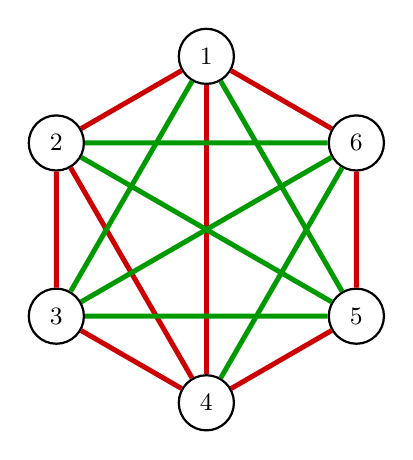
\begin{tikzpicture}[
    vertex/.style={circle, draw=black, fill=white, thick, minimum size=7mm, font=\small},
    red edge/.style={draw=red!80!black, line width=1.8pt},
    green edge/.style={draw=green!60!black, line width=1.8pt},
    scale=2.2
]
 
% --- Vertices arranged in a regular hexagon ---
\foreach \i/\label in {1/1, 2/2, 3/3, 4/4, 5/5, 6/6} {
    \node[vertex] (v\i) at ({90 + (\i-1)*60}:1) {\label};
}
 
% --- Edges (K_6: all 15 pairs) ---
% Colouring chosen so that:
%   Monochromatic RED triangle:   v1-v2-v4
%   Monochromatic GREEN triangle: v3-v5-v6 (and v1-v3-v5 is also green)
 
% Red edges
\draw[red edge] (v1)--(v2);
\draw[red edge] (v1)--(v4);
\draw[red edge] (v2)--(v4);
\draw[red edge] (v2)--(v3);
\draw[red edge] (v3)--(v4);
\draw[red edge] (v4)--(v5);
\draw[red edge] (v5)--(v6);
\draw[red edge] (v1)--(v6);
 
% Green edges
\draw[green edge] (v1)--(v3);
\draw[green edge] (v1)--(v5);
\draw[green edge] (v2)--(v5);
\draw[green edge] (v2)--(v6);
\draw[green edge] (v3)--(v5);
\draw[green edge] (v3)--(v6);
\draw[green edge] (v4)--(v6);
 
\end{tikzpicture}
\caption{An example 2-colour colouring fulfilling Ramsey number \( R(3,3)=6 \). Nodes 1, 3, 5 form a clique size 3. LaTeX code generated by Anthropic's Claude Sonnet 4.6}
\label{fig:ramsey33}
\end{figure}

On the other hand, below is a graph with 5 nodes where there are no monochromatic cliques, showing that \( R(3,3) > 5 \):

\begin{figure}[H]
\centering
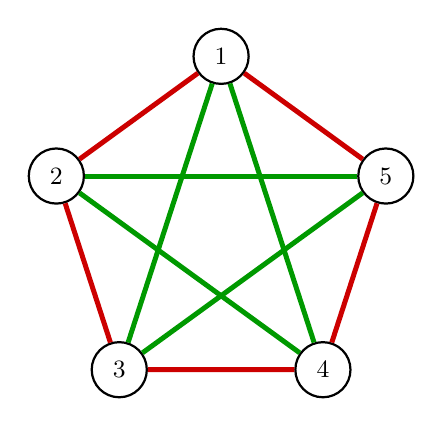
\begin{tikzpicture}[
    vertex/.style={circle, draw=black, fill=white, thick, minimum size=7mm, font=\small},
    red edge/.style={draw=red!80!black, line width=1.8pt},
    green edge/.style={draw=green!60!black, line width=1.8pt},
    scale=2.2
]
 
% --- Vertices arranged in a regular pentagon ---
\foreach \i in {1,...,5} {
    \node[vertex] (v\i) at ({90 + (\i-1)*72}:1) {\i};
}
 
% --- Red edges: outer pentagon cycle ---
\draw[red edge] (v1)--(v2);
\draw[red edge] (v2)--(v3);
\draw[red edge] (v3)--(v4);
\draw[red edge] (v4)--(v5);
\draw[red edge] (v5)--(v1);
 
% --- Green edges: inner pentagram (skip-one connections) ---
\draw[green edge] (v1)--(v3);
\draw[green edge] (v3)--(v5);
\draw[green edge] (v5)--(v2);
\draw[green edge] (v2)--(v4);
\draw[green edge] (v4)--(v1);
 
\end{tikzpicture}
\caption{An example 2-colour colouring showing how 5 nodes is not enough. \( R(3,3) > 5 \). There is no monochromatic clique. LaTeX code generated by Anthropic's Claude Sonnet 4.6}
\label{fig:ramsey33-k5}
\end{figure}

\subsection{Finding Lower Bounds of Ramsey Numbers}

To return to the probabilistic method and with the concept of Ramsey numbers explained here is the proof published by Erdős in 1947 \autocite{erdosRemarksTheoryGraphs1947} \autocite{alonProbabilisticMethod2008}:

\begin{theorem}[Erdős 1947] \label{thm:erdos-1947}
    If \( \binom{n}{k} \times 2^{1-\binom{k}{2}} < 1 \) then \( R(k,k) > n \)
\end{theorem}    

\begin{proof}
    Let's start by colouring the edges of a complete graph on \( K_n \) nodes using two colours uniformly at random. The edges are coloured of equal probability:
    \[
        P(\text{an edge is red}) = P(\text{an edge is green}) = \frac{1}{2}
    \] 
    
There are k (from our diagonal Ramsey number \( R(k,k)\)) nodes from n total nodes we want to pick from meaning we can apply the formula from section \ref{sec:combinations-permutations}: 
\[
    \frac{n!}{r!(n-r)!} = \binom{n}{r} = \binom{n}{k}
\]

Next, let's define an event, \( A_S \) in which a clique \( S \) of size k is monochromatic. In other words, a subgraph which has k nodes of our initial graph \( K_n \) of a single colour. The probability of that occurring is:

\[
    P(A_S) = 2 \times \left(\frac{1}{2}\right)^{\binom{k}{2}}
\]
Where the leading two is there because we do not care about which of the two colours the clique has. The \( \frac{1}{2} \) stems from the initial probability of the colouring of the edges. And the \( \binom{k}{2} \) defines all possible edges in the clique, i.e. all pairs of nodes. We can simplify this to:

\[
    P(A_S) = 2 \times \left(\frac{1}{2}\right)^{\binom{k}{2}} = 2 \times 2^{-\binom{k}{2}} = 2^{1-\binom{k}{2}}
\]

Since there are \( \binom{n}{k} \) possible arrangements of the clique size k, we can then multiply that to find the probability of any clique of size k of any colour to be monochromatic:

\begin{equation} \label{eq:union-bound-clique}
   P(\text{there exists a monochromatic clique } K_k) \leq \binom{n}{k} \times 2^{1-\binom{k}{2}}
\end{equation}

By the assumption of the theorem, however, we know that:
\[
    \binom{n}{k} \times 2^{1-\binom{k}{2}} < 1 
\]
And therefore there is a positive probability that there exists such a graph for a complete graph \( K_n \):
\[
    P(\text{there does not exist a monochromatic clique } K_k) > 0
\]
If that is the case, we have not yet achieved the requirements of a Ramsey number which is the absence of the possibility that \textit{there does not exist a monochromatic clique} which is why:
\[
    R(k,k) > n
\]
For n which we chose at the beginning of the proof.


\end{proof}




\section{Predicting clique sizes in Scale Free Networks} \label{sec:predicting-clique-sizes}
% -	Setting out the problem: we want to find specific clique sizes in a scale free network with 4 hubs
% -	Using the first moment we will explain the concept of 

With both the concepts of scale free networks and the probabilistic method explained, we can now move on to the core of this essay. If we conceptually combine them both, trying to find a relation between clique sizes and the coefficient \( \gamma \) we expect an inverse relationship between the two since a lower \( \gamma \) value has shown to increase the density of the graph. A paper by \autocite{bianconiNumberCliquesRandom2006} comes to the following derivation (the notation has been slightly adapted to fit the rest of this essay):


\begin{equation} \label{eq:bianconi-marsili-bound}
    \bar{c} \simeq \sqrt{b}\, n^{\frac{3-\gamma}{4}}
\end{equation}

Where \( \bar{c} \) is the upper limit to the clique size, \( n \) is the number of nodes, \( \gamma \) stays the same, \( b \) is a new parameter which I will introduce below and \( c \) is the actual clique size of the graph. 

The authors of the paper define the constant \( b \) to be:
\begin{equation} \label{eq:b-original-bianconi-marsili}
b = (\gamma - 1)\, m^{\gamma - 1}\, e\, \langle q \rangle^{\frac{1-\gamma}{2}}
\end{equation}

Adapted to the notation consistent with this essay:

\begin{equation} \label{eq:b-adapted}
b = (\gamma - 1)\, w_{\text{min}}^{\gamma - 1}\, e\, \left (\frac{S}{n} \right ) ^{\frac{1-\gamma}{2}}
\end{equation}

Although not immediately introduced, \( w_{\text{min}} \) can be directly derived from \( w_{\text{max}} \) as \textcite{fasinoGeneratingLargeScalefree2021} show:

\begin{equation} \label{eq:wmax-wmin-relation}
    w_{\text{max}} \approx w_{\text{min}}\, n^{\frac{1}{\gamma - 1}}
\end{equation}

Rearranging to:
\[
    w_{\text{min}} \approx w_{\text{max}}\, n^{-\frac{1}{\gamma - 1}}
\]


Putting everything together:
\[
    b = (\gamma - 1) \left ( w_{\text{max}}\, n^{-\frac{1}{\gamma - 1}} \right )^{\gamma - 1}\, e \left (\frac{S}{n} \right ) ^{\frac{1-\gamma}{2}}
\]

Which simplifies to:
\begin{equation} \label{eq:b-simplified}
    b = (\gamma - 1)  \frac{w_{\text{max}}^{\gamma - 1}}{n} \, e \left (\frac{S}{n} \right ) ^{\frac{1-\gamma}{2}}
\end{equation}

As a reminder:

\[
w_{\text{max}} = \sum_{i}{i^{ -\frac{1}{\gamma-1}}}
\]




In other words, to move forward predicting the next step, we need to define \( \gamma \) and \( n \)



\begin{table}[H]
\centering
\label{tab:params-initial}
\begin{tabular}{c c}
\toprule
{Variable} & {Value}  \\
\midrule
\( \gamma \) & 2.4 \\
\( n \) & 1000 \\
\bottomrule
\end{tabular}
\caption{}
\end{table}

We can then calculate \( w_{\text{max}} \):

\[
w_{\text{max}} = \sum_{i=1}^{n}{i^{ -\frac{1}{\gamma-1}}} = \sum_{i=1}^{1000}{i^{ -\frac{1}{2.4-1}}} = 22.248620809477696
\]

And then calculate \( b \), assuming \( w_{\text{max}}^2 = S \):

\[
 b = (\gamma - 1)  \frac{w_{\text{max}}^{\gamma - 1}}{n} \, e \left (\frac{S}{n} \right ) ^{\frac{1-\gamma}{2}} = (2.4 - 1)  \frac{10.121^{2.4 - 1}}{1000} \, e \left (\frac{10.121^2}{1000} \right ) ^{\frac{1-2.4}{2}} = 0.4790959698
\]

We can then update the table:

\begin{table}[H]
\centering
\label{tab:params-updated}
\begin{tabular}{c c}
\toprule
{Variable} & {Value}  \\
\midrule
\( \gamma \) & 2.4 \\
\( n \) & 1000 \\
\( b \) & 0.9559509674 \\
\bottomrule
\end{tabular}
\caption{}
\end{table}


And insert all the variables:
\[
    \bar{c} \simeq \sqrt{b}\, n^{\frac{3-\gamma}{4}} = \sqrt{0.9559509674}\, 1000^{\frac{3-2.4}{4}} = 1.950822736
\]

In other words, we predict that when we set \( w_{\text{min}} = 0.005 \) then the maximal clique size at \( \gamma = 2.4 \) in a scale free network with \( n = \num{1000} \) nodes is 2 since a clique size needs to be an integer. 

This number is tightly bound, however, because we have to reflect the bounds on the parameters and the statistical meaning. The authors set a boundary of \( \epsilon \in 0,1 \) and \( \gamma \in 2,3 \) as both of these change random generation drastically if outside the bounds. Furthermore, if the graph is not dense enough, it will become nearly impossible to work with probabilities correctly as there is no meaningful number of edges that could generate a clique and therefore show the same prediction. At \( \gamma = 2.4 \) we can assume the edge density to be meaningful enough, however any greater makes the \( n = \num{10000} \) node graph have a density of less than \( 1 \% \). 
Specifically for this reason the generation of the scale free networks in the next section will make use of a very high \( w_{\text{min}} \) value which will lead to high clipping rates as discussed in section \ref{sec:scale-free-networks}. These are, however, necessary because the limited computing power available to me limits the maximum nodes I can generate en masse.
As a result this essay is taking an empirical approach to find a relation between \( \gamma \) and maximal clique sizes.

\section{Building Scale Free Networks}
% -	Using the help of AI to code a python script, I aim to generate a statistically meaningful number of Scale-Free Networks.
% -	By analysing the sizes of clique’s present, I should be able to find similar results to my theoretical/probabilistic approach
% - Create another example similar to the walkthrough

% The theoretical derivation from section \ref{sec:predicting-clique-sizes} shows the inversely proportional relationship between the degree power coefficient \( \gamma \) and the maximum clique size of a scale free network.

To generate the random scale free networks required to empirically explore these graphs, I instructed Claude Sonnet 5 to generate a python script which sweeps through \( \gamma \) values 2.0 to 3 taking steps of 0.05. The script generated a total of \(\num{10500000}\) graphs with \( n =100\) through \( n =100\) nodes each, generating \(\num{50000}\) different graphs per \( \gamma \) value. I then plotted the bivariate relationship between \( \gamma \) and maximal clique size on a coordinate plane which is presented in section \ref{sec:presenting-understanding-results} after the following explanation. 

For the reader to understand the generation process the following part will build a much smaller scale free network on paper. 

Let's generate a graph of \( n=5 \) nodes with gamma coefficient \( \gamma = 2.3 \). First we need to generate the relevant weights attributed to every node. From the \textit{cite the paper here} we know to use equation \ref{eq:weight-generation-equation} from section \ref{sec:scale-free-networks}

\[
    w_i = w_{\text{max}} \times i^{ -\frac{1}{\gamma-1}}
\]

The first step is to calculate the largest possible \( w_{\text{max}} \). From equation \ref{eq:wmax-leq-T} we know: 

\[
w_{\text{max}} \leq \sum_{i}{i^{ -\frac{1}{\gamma-1}}}
\]
Inserting the variables: 
\[
w_{\text{max}} = \sum_{i = 5}{i^{ -\frac{1}{2.3-1}}} 
\]
And calculating using Excel:
\[
w_{\text{max}} = 2.650457959
\]

Next we have to calculate the weight of every node. To simplify these steps, we can make the exponent \( \frac{1}{\gamma-1} \) a constant:

\[ \alpha = \frac{1}{\gamma-1} = \frac{1}{2.3-1} = 0.7692307692 \]

And build a table calculating every step:




\begin{table}[htbp]
\centering
\label{tab:rank-weights}
\begin{tabular}{c S[table-format=1.3] S[table-format=1.3] S[table-format=1.3]}
\toprule
{rank \(i\)} & {\(w_{\text{max}}\)} & {\(i^{-\alpha}\)} & {\(w_i = w_{\text{max}} \times i^{-\alpha}\)} \\
\midrule
1 & 2.650 & 1.000 & 2.650 \\
2 & 2.650 & 0.587 & 1.555 \\
3 & 2.650 & 0.430 & 1.138 \\
4 & 2.650 & 0.344 & 0.912 \\
5 & 2.650 & 0.290 & 0.769 \\
\bottomrule
\end{tabular}
\caption{}
\end{table}

Next we need to allocate a weight to every node,  for simplicity the rank and node will stay the same, meaning we end up with the following information: 


\begin{table}[htbp]
\centering
\label{tab:node-weight-allocation}
\begin{tabular}{c S[table-format=1.3] S[table-format=1.3]}
\toprule
{rank \(i\)} & {node \( v_i \)} & {weight \( w_i \)} \\
\midrule
1 & 1 & 2.650 \\
2 & 2 & 1.555 \\
3 & 3 & 1.138 \\
4 & 4 & 0.912 \\
5 & 5 & 0.769 \\
\bottomrule
\end{tabular}
\caption{}
\end{table}

With the node weights generated we can calculate the probabilities of generating an edge between two nodes. For that we follow equation \ref{eq:chung-lu-conf-model}:

\[
    p_{hj} = \frac{w_h w_j}{\sum_{i}{w_i}}
\]
We can first calculate \( \sum_{i}{w_i} \) by summing up all weights:

\[ 
2.650+1.555+1.138+0.912+0.769 = 7.025
\]

This also allows us to check whether the weights are feasible:

\[
w_{\text{max}}^2< \sum_{i}{w_i} = 2.650^2 < 7.02492739 = 7.02492739
\]

Since we decided to take the largest possible value for \( w_{\text{max}} \) following the equality from before, we are now faced with the fact that the graph, specifically the node with the largest weight would have a guaranteed loop. Since we are working with simple graphs, however, there are no loops meaning that this is not a problem.

We can then calculate all weight products:

\begin{table}[H]
  \centering
  \label{tab:calculated-probabilities-step-1}
  \begin{tabular}{c S[table-format=2.3] S[table-format=2.3] S[table-format=2.3] S[table-format=2.3] S[table-format=2.3]}
    \toprule
    {} & {\(w_1 = 2.650\)} & {\(w_2 = 1.555\)} & {\(w_3 = 1.138\)} & {\(w_4 = 0.912\)} & {\(w_5 = 0.769\)} \\
    \midrule
    \(w_1 = 2.650\) & {} & 4.122 & 3.017 & 2.418 & 2.037 \\
    \(w_2 = 1.555\) & 4.122 & {} & 1.770 & 1.419 & 1.195 \\
    \(w_3 = 1.138\) & 3.017 & 1.770 & {} & 1.039 & 0.875 \\
    \(w_4 = 0.912\) & 2.418 & 1.419 & 1.039 & {} & 0.701 \\
    \(w_5 = 0.769\) & 2.037 & 1.195 & 0.875 & 0.701 & {} \\
    \bottomrule
  \end{tabular}
  \caption{Pairwise products of weights}
\end{table}

As a reminder, we are not multiplying the weights by themselves because we are not interested in loops.

We can then divide by the sum of all weights \( \sum_{i}{w_i}=7.025 \):

\begin{table}[htbp]
  \centering
  
  \label{tab:calculated-probabilities-step-2}
  \begin{tabular}{c S[table-format=1.3] S[table-format=1.3] S[table-format=1.3] S[table-format=1.3] S[table-format=1.3]}
    \toprule
    {} & 
    {\(\frac{w_1}{\sum_i w_i} = \frac{2.650}{7.025}\)} & 
    {\(\frac{w_2}{\sum_i w_i} = \frac{1.555}{7.025}\)} & 
    {\(\frac{w_3}{\sum_i w_i} = \frac{1.138}{7.025}\)} & 
    {\(\frac{w_4}{\sum_i w_i} = \frac{0.912}{7.025}\)} & 
    {\(\frac{w_5}{\sum_i w_i} = \frac{0.769}{7.025}\)} \\
    \midrule
    \(w_1 = 2.650\) & {}          & 0.587   & 0.430   & 0.344   & 0.290   \\
    \(w_2 = 1.555\) & 0.587   & {}            & 0.252 & 0.202   & 0.170   \\
    \(w_3 = 1.138\) & 0.430   & 0.252   & {}          & 0.148   & 0.125   \\
    \(w_4 = 0.912\) & 0.344   & 0.202   & 0.148   & {}          & 0.100   \\
    \(w_5 = 0.769\) & 0.290   & 0.170   & 0.125   & 0.100   & {}          \\


    \bottomrule
  \end{tabular}
  \caption{Pairwise products of normalized weights}
\end{table}

We now have the theoretical probability of an edge between every node in our graph.
We can now generate the actual edges. In the script, a random value is generated between 0 and 1 and if it is less than the value, an edge is placed. For the purpose of this demonstration Excel generated the values. As a reminder, node \(v_i \) has weight \(w_i\).

\begin{table}[H]
  \centering
  \label{tab:edge-realization-2}
  \begin{tabular}{c S[table-format=1.3] c l}
    \toprule
    {Pair} & {\(P_{hj}\)} & {Random Value} & {Edge?} \\
    \midrule
    \((1,2)\) & 0.587 & 0.209 & TRUE  \\
    \((1,3)\) & 0.430 & 0.465 & FALSE \\
    \((1,4)\) & 0.344 & 0.154 & TRUE  \\
    \((1,5)\) & 0.290 & 0.358 & FALSE \\
    \((2,3)\) & 0.252 & 0.741 & FALSE \\
    \((2,4)\) & 0.202 & 0.125 & TRUE  \\
    \((2,5)\) & 0.170 & 0.834 & FALSE \\
    \((3,4)\) & 0.148 & 0.010 & TRUE  \\
    \((3,5)\) & 0.125 & 0.474 & FALSE \\
    \((4,5)\) & 0.100 & 0.237 & FALSE \\

    \bottomrule
  \end{tabular}
  \caption{Edge realization for each node pair}
\end{table}

If we were to draw it, this would be the result:

\begin{figure}[H]
\centering
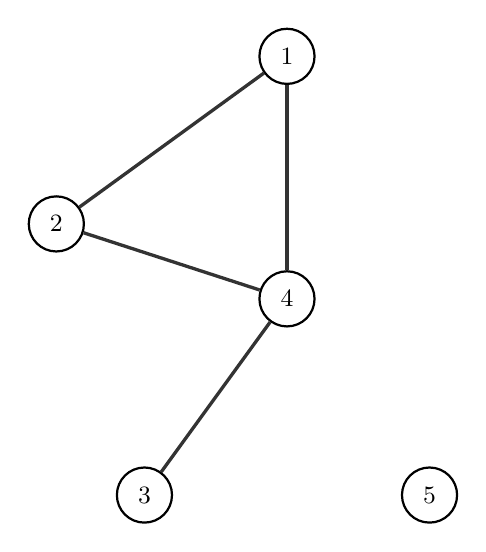
\begin{tikzpicture}[
    vertex/.style={circle, draw=black, fill=white, thick, minimum size=7mm, font=\small},
    edge/.style={draw=black!80, line width=1.2pt},
    scale=2.2
]

% --- Hub vertex (highest degree) at center ---
\node[vertex] (v4) at (0,0) {4};

% --- Remaining vertices on outer ring, ordered by descending degree ---
% Degrees: v4=3 (hub), v1=2, v2=2, v3=1, v5=0
\node[vertex] (v1) at (90:1.4)  {1};
\node[vertex] (v2) at (162:1.4) {2};
\node[vertex] (v3) at (234:1.4) {3};
\node[vertex] (v5) at (306:1.4) {5};

% --- Edges realized ---
% Present: (1,2) (1,4) (2,4) (3,4)
% Absent:  (1,3) (1,5) (2,3) (2,5) (3,5) (4,5)

\draw[edge] (v1)--(v2);
\draw[edge] (v1)--(v4);
\draw[edge] (v2)--(v4);
\draw[edge] (v3)--(v4);

\end{tikzpicture}
\caption{Realized graph from the Chung-Lu edge probability trial, with the hub vertex (degree 4) placed at the center. LaTeX code generated by Anthropic's Claude Sonnet 5}
\label{fig:chung-lu-realization-3}
\end{figure}

\section{Presenting and Understanding Results} \label{sec:presenting-understanding-results}
% -	Comparing results and making sure theory aligns with empirical data
% \cite{jursaCliqueNumberEstimates2020}
% \textit{Since I was not able to write out section 5, I cannot compare anything}

% After generating a statistically meaningful number of graphs we can conclude that empirical data is in line with literature. The small deviation in maximal clique sizes can be explained by the findings of \textit{cite here} paper. It is important to note, however, that there is a large number of 

The generation of a statistically meaningful number of graphs means we can empirically make conclusions about relationships between \( \gamma \) and the maximal clique size \( c \). As a reminder, I generated a total of \(\num{10500000}\) graphs with \( n =100\) through \( n =1000\) nodes each, generating \(\num{50000}\) different graphs per \( \gamma \) value. 

It seems like \( c \) follows a quadratic relationship to \( \gamma \). This relationship holds at an \( R^2 = 0.9675 \text{ to } 0.9995 \), depending on the number of nodes, \(n\) greater than any other common relationship. Figure below shows the value for \(n=100\).

\begin{figure}[H]
\centering
\begin{subfigure}[b]{0.48\textwidth}
    \centering
    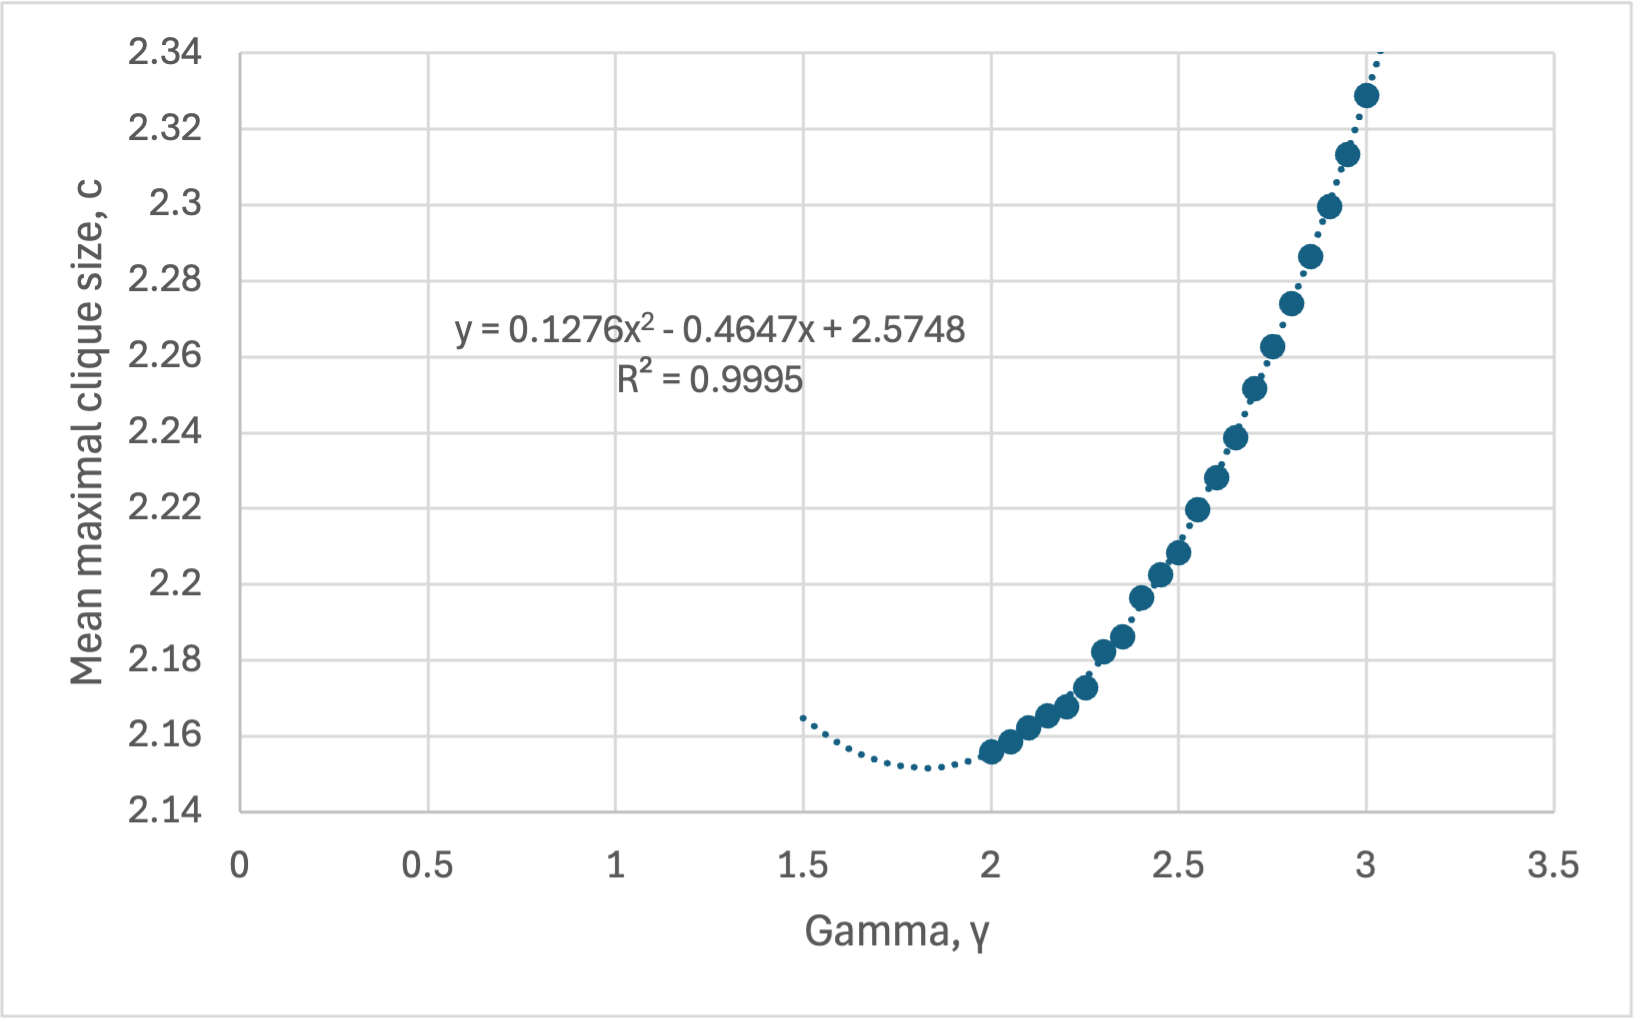
\includegraphics[width=\textwidth]{n100GammaClique.png}
    \caption{First image caption}
    \label{fig:sub1}
\end{subfigure}
\hfill
\begin{subfigure}[b]{0.48\textwidth}
    \centering
    \includegraphics[width=\textwidth]{n1000GammaClique.png}
    \caption{Second image caption}
    \label{fig:sub2}
\end{subfigure}
\caption{Overall caption describing both}
\label{fig:both}
\end{figure}

More notably, this relationship shifts on the coordinate plane as \(n\) changes. Bringing together all generated quadratic equations onto a single coordinate plane gives us the following figure, where the red zone is the scope which this essay has been looking at: 

\begin{figure}[H]
\centering
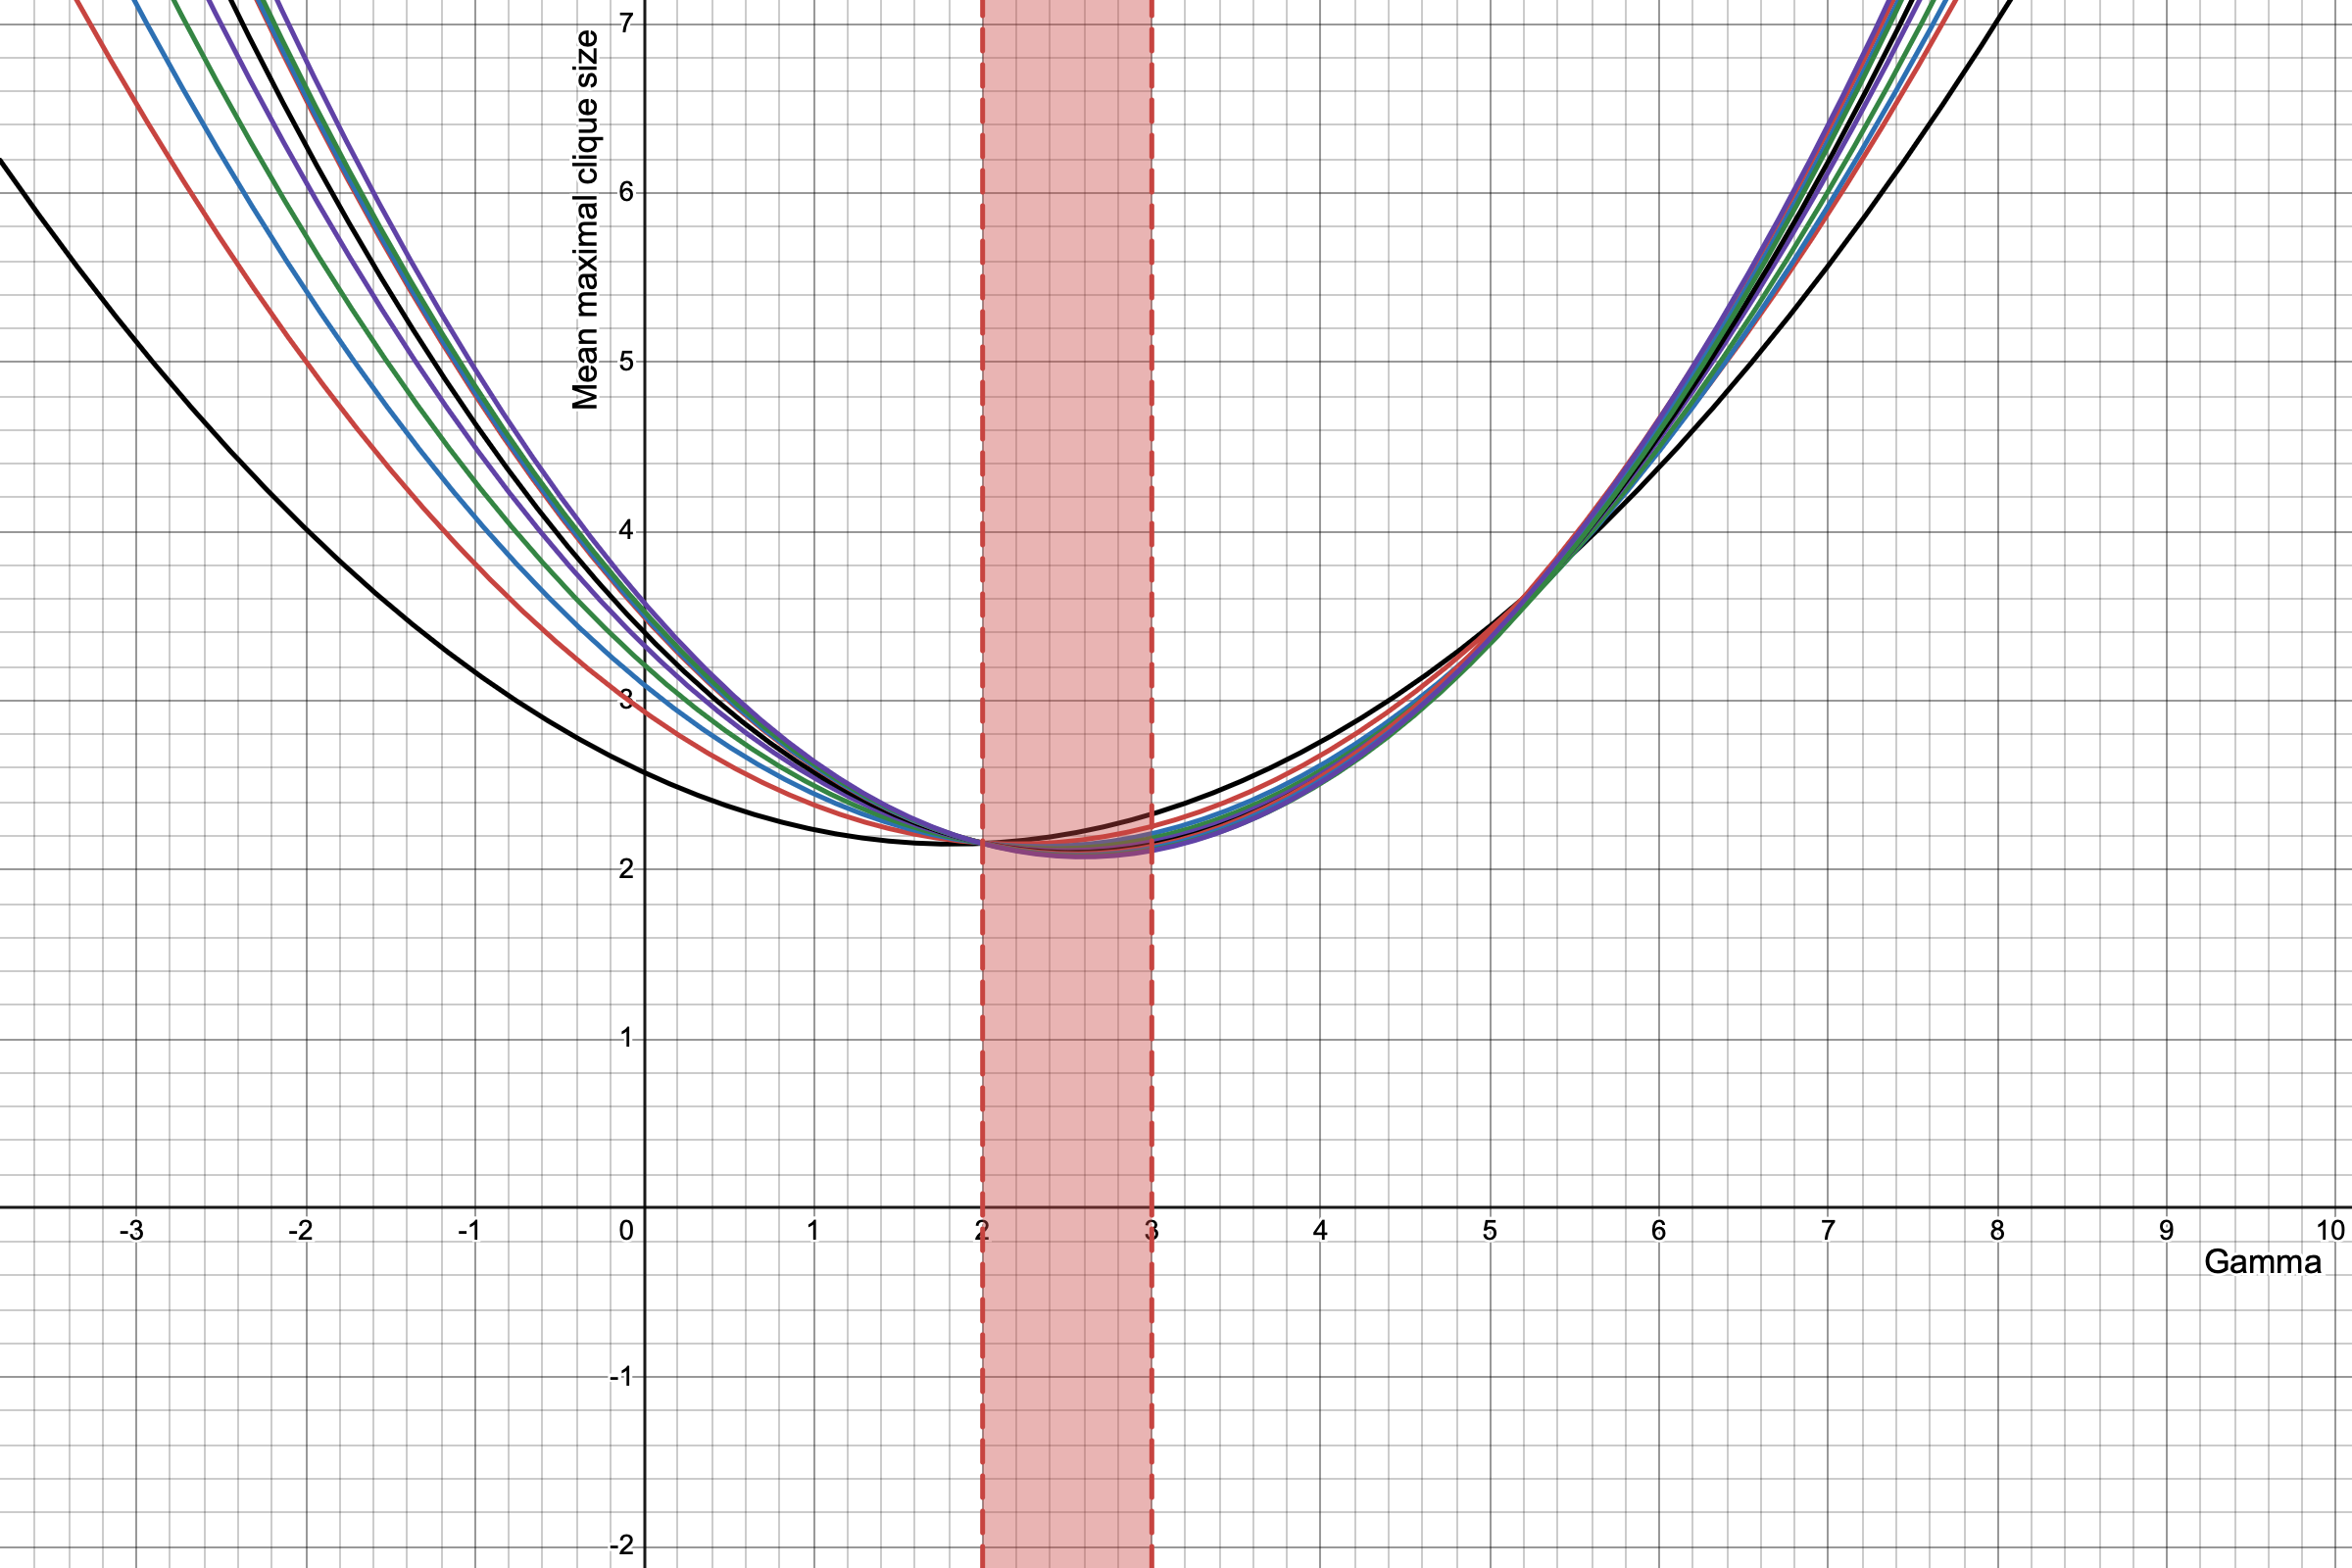
\includegraphics[width=0.48\textwidth]{allNGammClique.png}
\caption{Caption text here}
\label{fig:my-image}
\end{figure}

Zooming in to better distinguish the individual curves, we notice how all of them seem to join on a point at the \( x =2 \) line:

\begin{figure}[H]
\centering
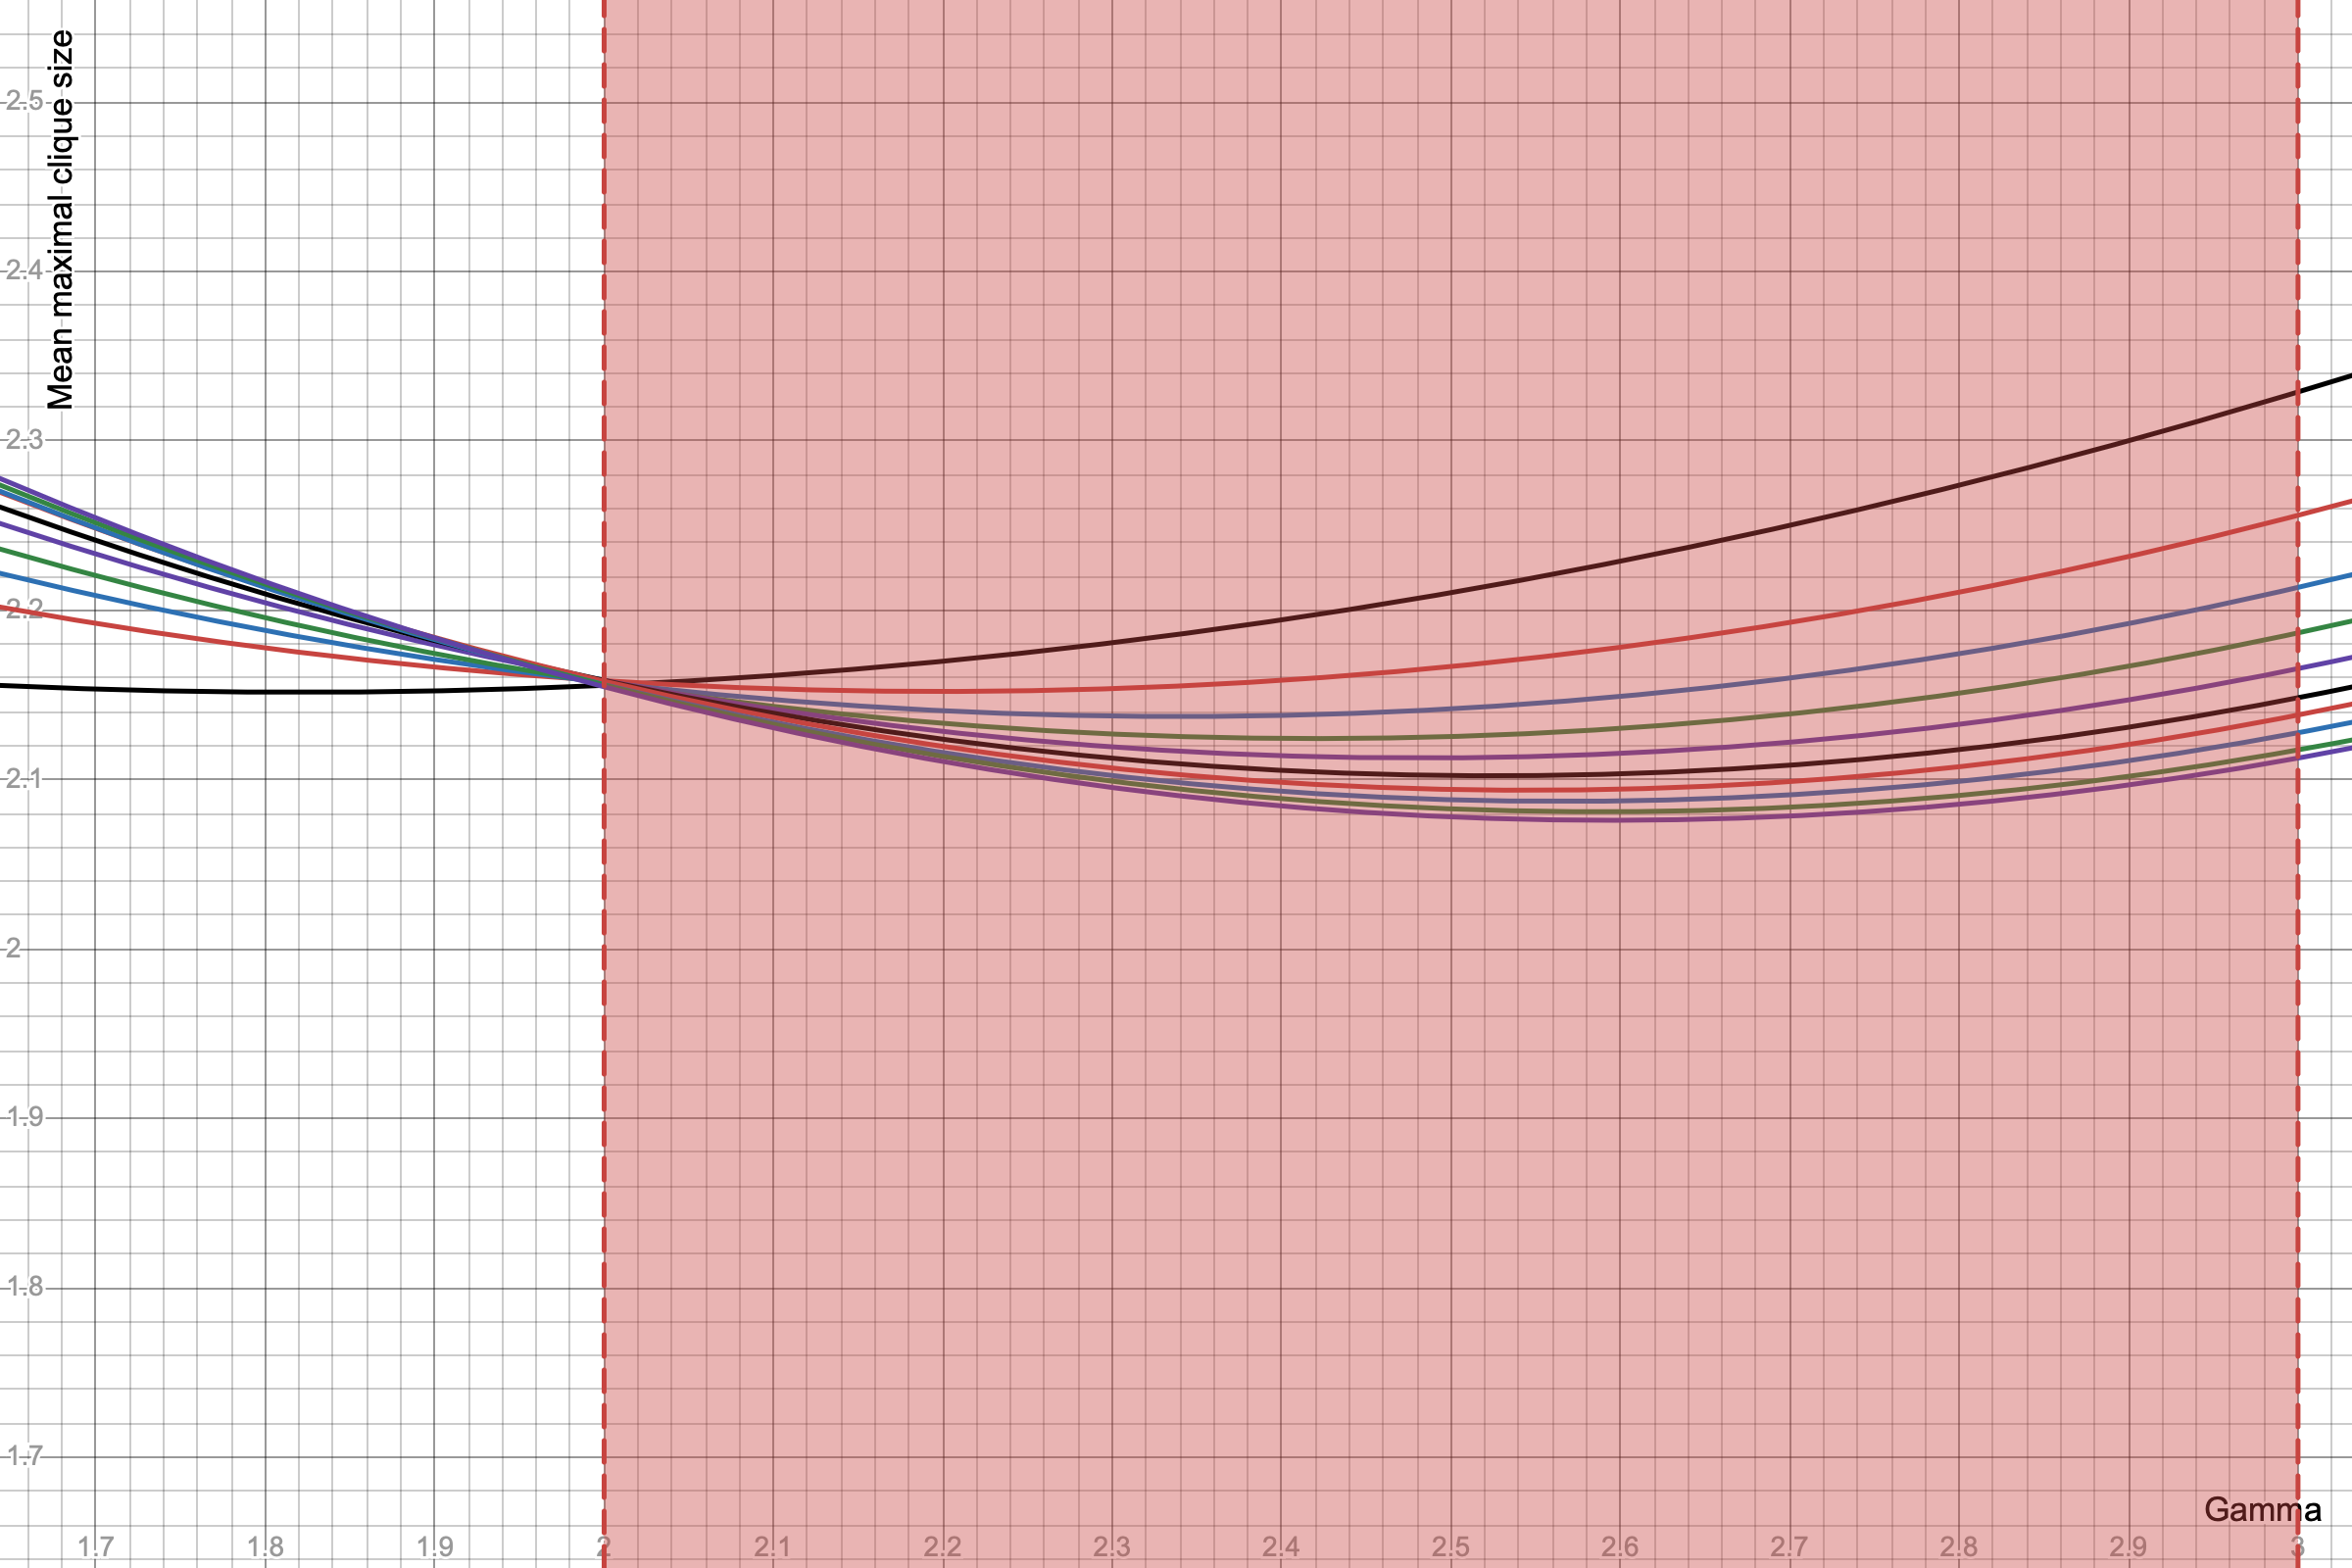
\includegraphics[width=0.48\textwidth]{allNZoomGammaClique.png}
\caption{Caption text here}
\label{fig:my-image}
\end{figure}

Although not doing so perfectly, this point is also the vertex of a quadratic equation shaped from the vertex points of all the other curves as seen below:

\begin{figure}[H]
\centering
\begin{subfigure}[b]{0.48\textwidth}
    \centering
    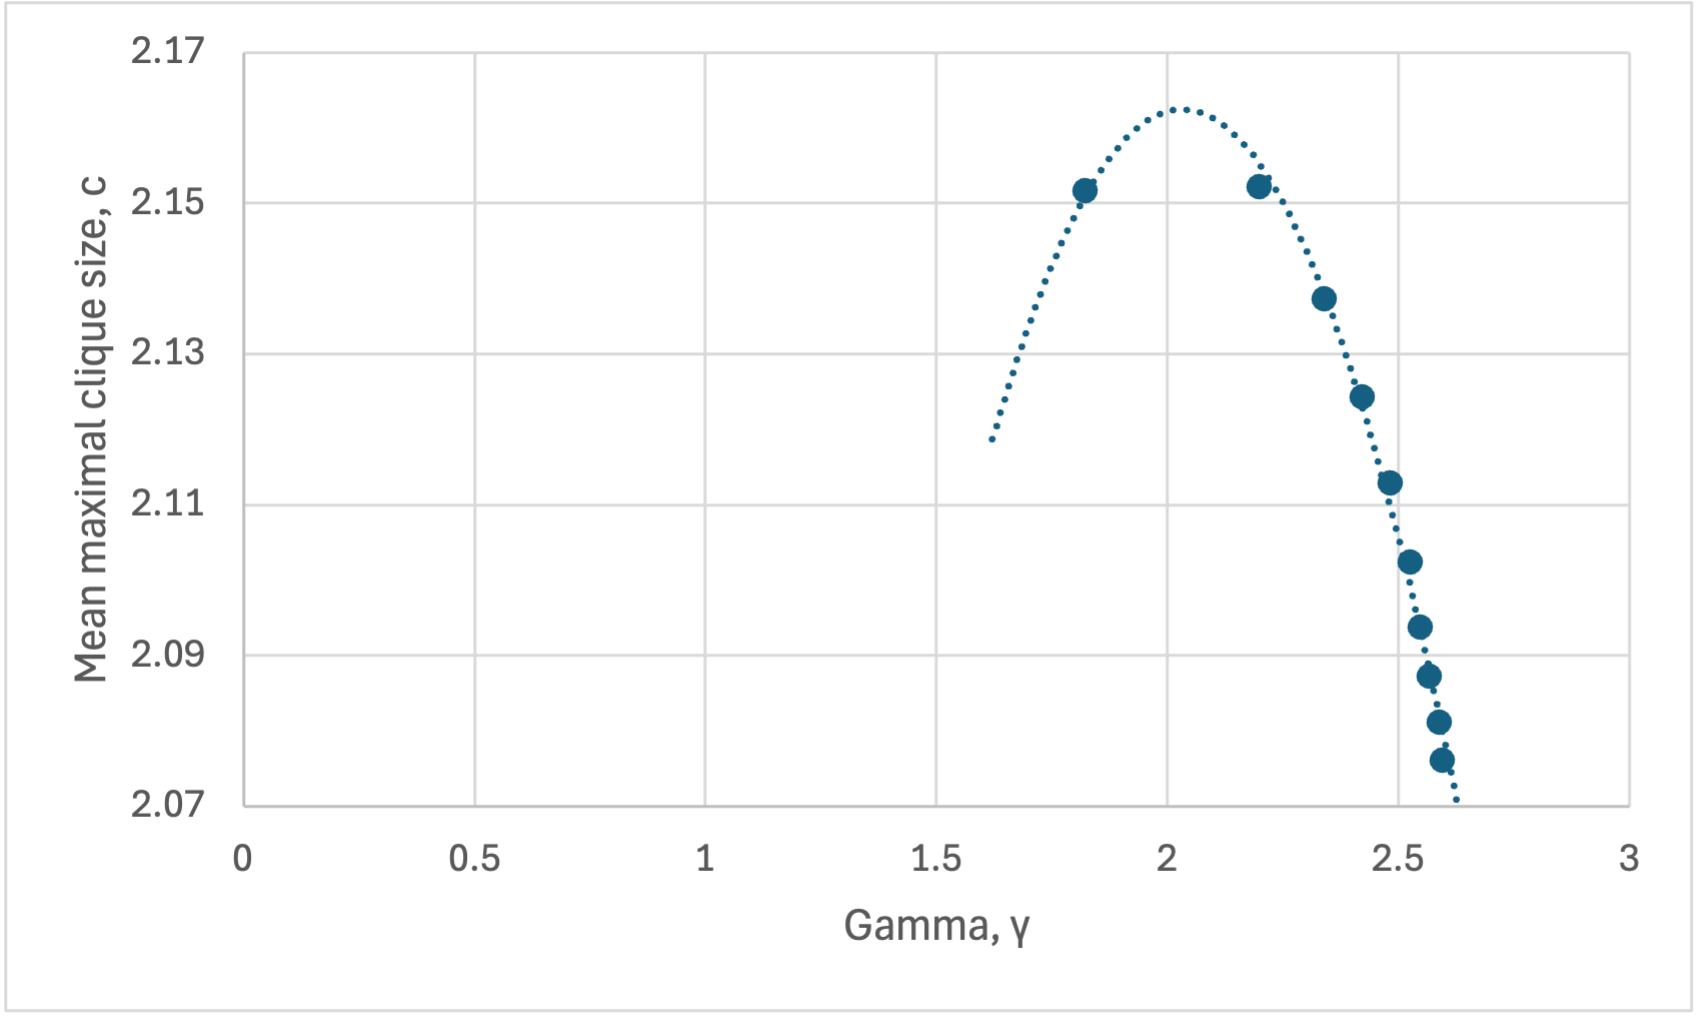
\includegraphics[width=\textwidth]{allNGammaCliqueVertex.png}
    \caption{First image caption}
    \label{fig:sub1}
\end{subfigure}
\hfill
\begin{subfigure}[b]{0.48\textwidth}
    \centering
    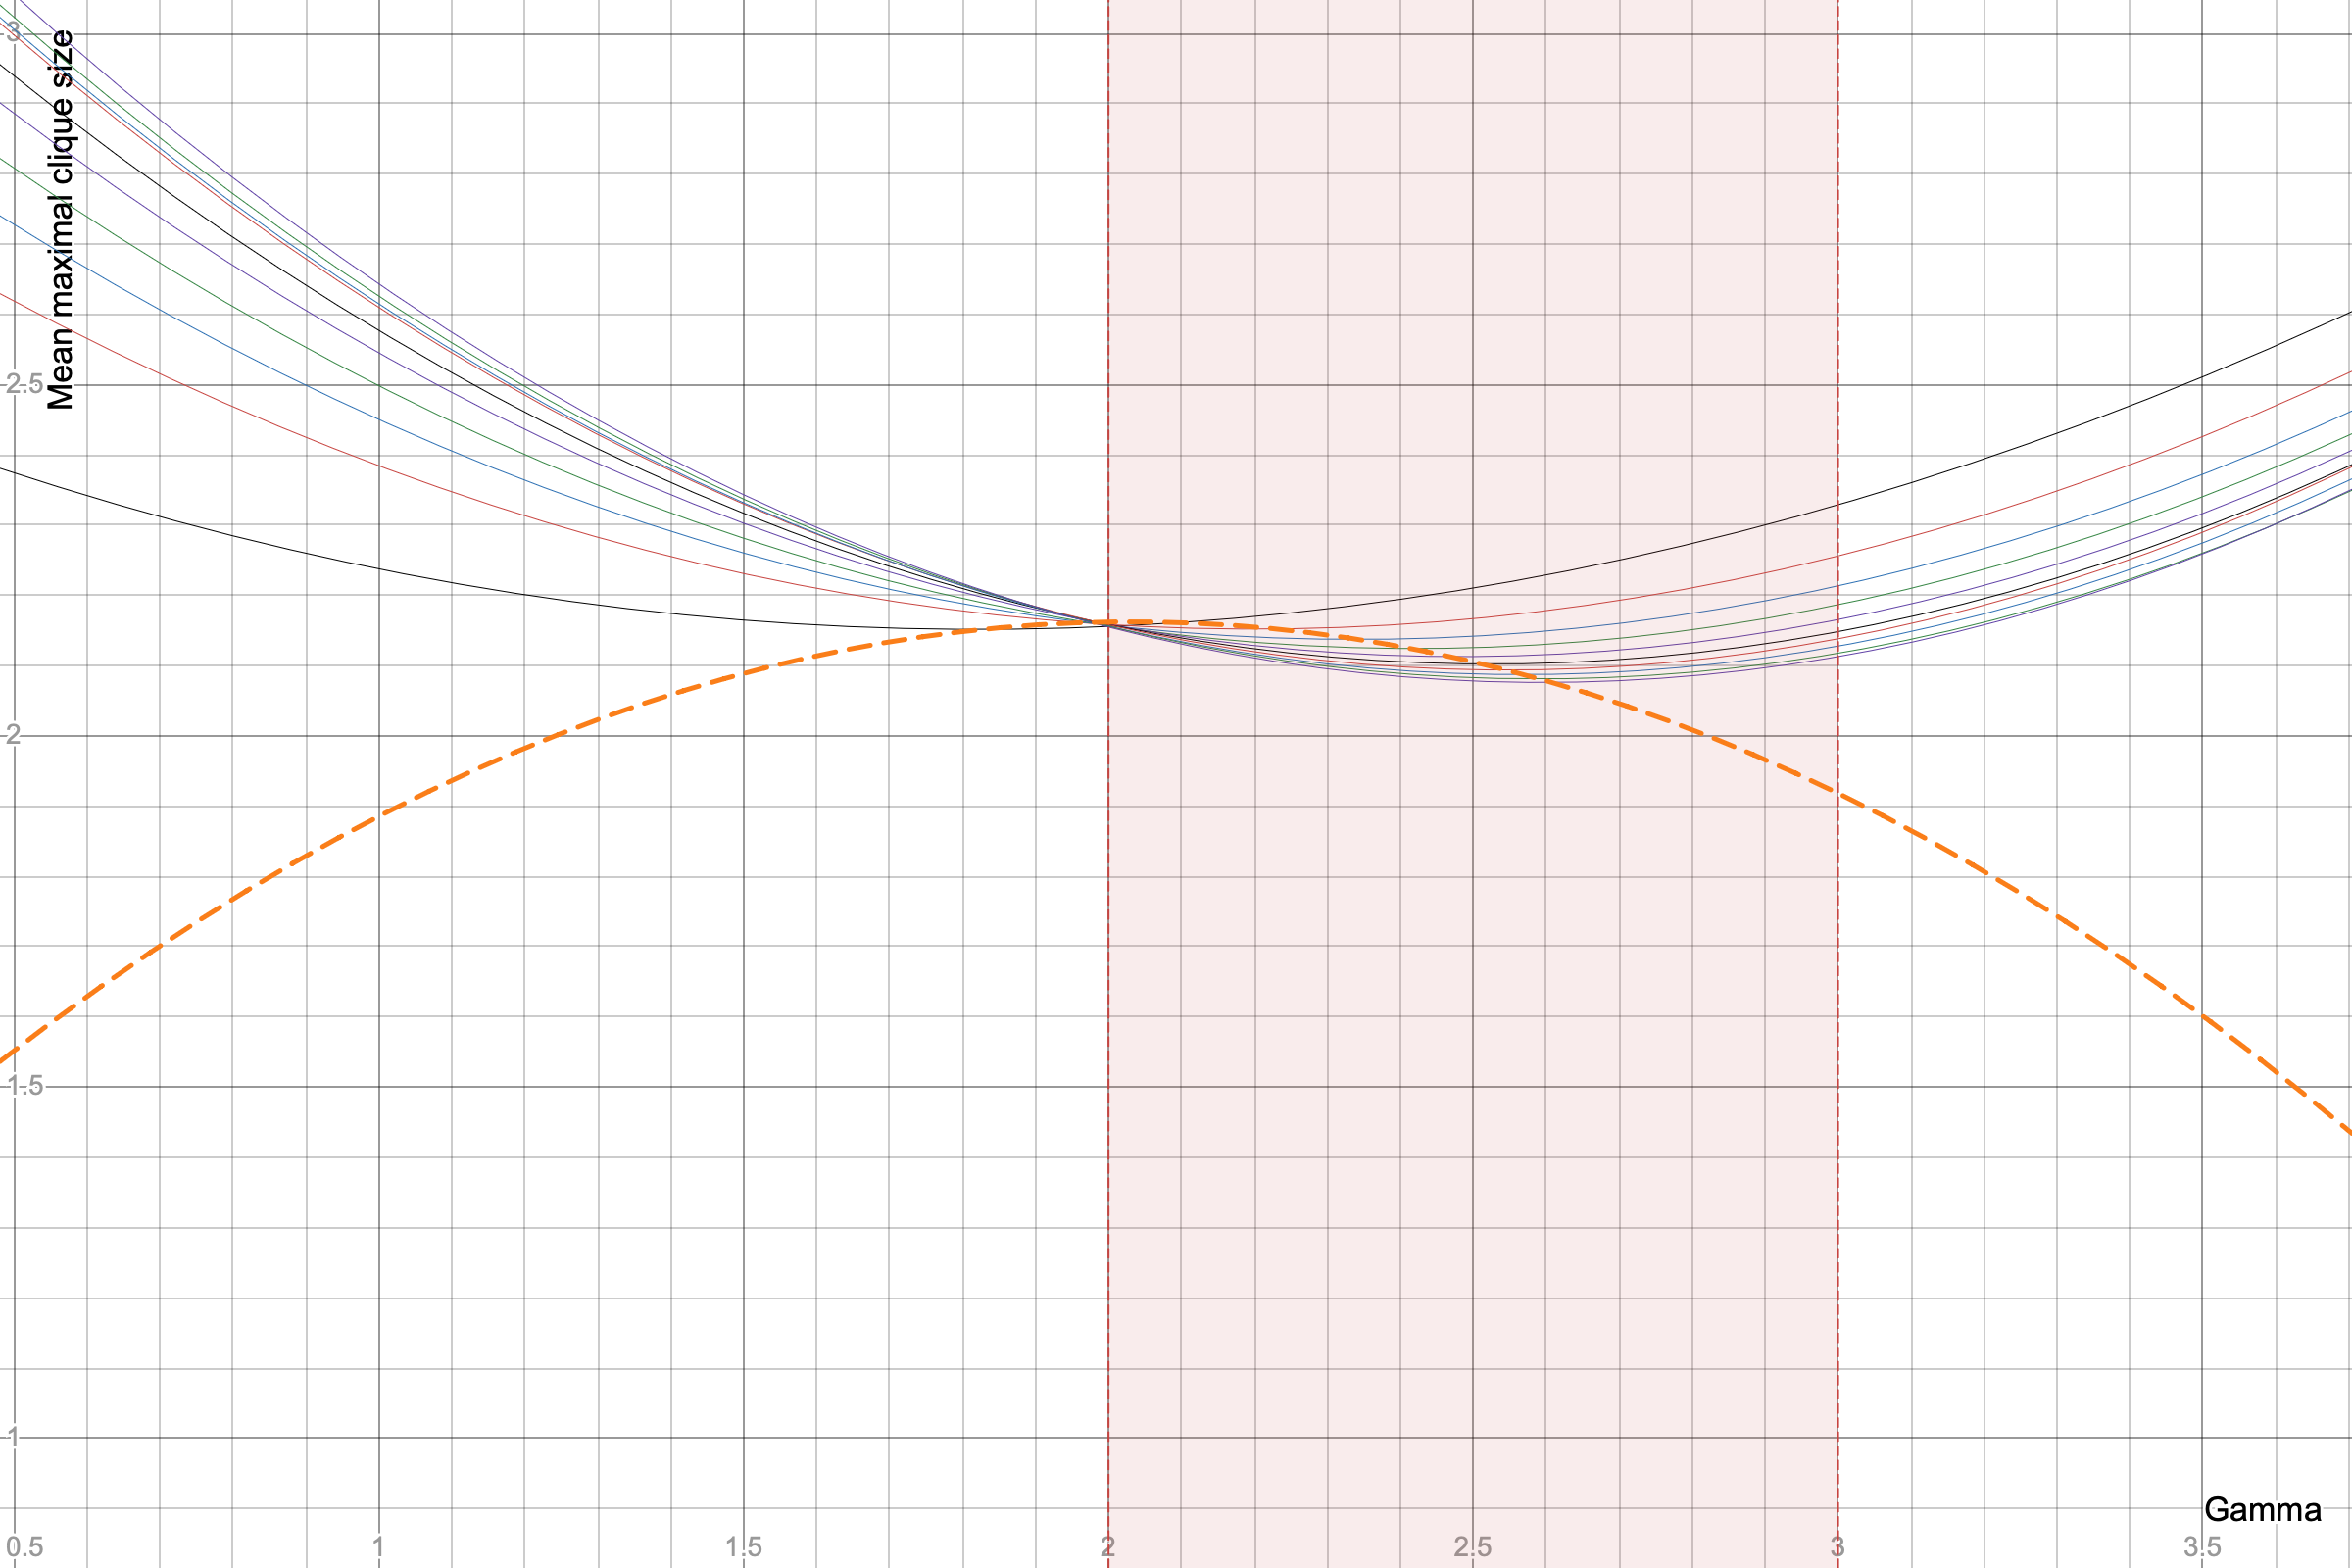
\includegraphics[width=\textwidth]{allNGammaCliqueParabola.png}
    \caption{Second image caption}
    \label{fig:sub2}
\end{subfigure}
\caption{Overall caption describing both}
\label{fig:both}
\end{figure}

To keep generations comparable, the maximum weight \(w_{\text{max}}\) was kept constant across all values of \(\gamma\). The maximum weight \(w_{\text{max}}\) was, however, not kept constant across values of \(n\). Following from equation \ref{eq:wmax-leq-T} in section \ref{sec:scale-free-networks}, the greater the \(n\) value, the greater the maximum weight. By changing \(w_{\text{max}}\) we could make sure these graphs were always generated at the edge of admissibility. 




\cite{jursaCliqueNumberEstimates2020}
\section{Conclusion}
% -	Conclude on the uses of my results
% To conclude, the application of scale free networks is very useful in the real world which makes them worth exploring both through an abstract and applicative lens. Through the use of the probabilistic method it is possible to predict patterns in randomly generated scale free networks which can then be applied to real world graphs such as large social media networks, or telecommunications optimisation problems. It is remarkable how these highly specific concepts dictate our every day lives in which very few people can imagine. 

With an understanding of the inverse relationship between \( \gamma \) and clique sizes we can estimate how interconnected we expect a certain graph can be. As power law distributions are common in nature, this information is vital to make simple initial estimates of the \( \gamma \) coefficient if we have a clique size, and vice versa if we have \( \gamma \). Although not mathematically rigorous, this information can then be further used to apply other statistical or mathematical methods to analyse graphs such as the internet, AWS 


\printbibliography[title={Works Cited}]




\end{document}